\documentclass[nojss]{jss}
\usepackage{bm,booktabs}
\usepackage{amsmath}
\usepackage{thumbpdf}
%% need no \usepackage{Sweave.sty}


\title{VAR, SVAR and SVEC Models: Implementation Within \proglang{R}
  Package \pkg{vars}}
\Plaintitle{VAR, SVAR and SVEC Models: Implementation Within R Package vars}
\Shorttitle{\pkg{vars}: VAR, SVAR and SVEC Models in \proglang{R}}

\author{Bernhard Pfaff\\Kronberg im Taunus}
\Plainauthor{Bernhard Pfaff}

\Abstract{
The structure of the package \pkg{vars} and its implementation of
vector autoregressive-, structural vector autoregressive- and
structural vector error correction models are explained in this
paper. In addition to the three cornerstone functions \code{VAR()},
\code{SVAR()} and \code{SVEC()} for estimating such models, functions
for diagnostic testing, estimation of a restricted models, prediction,
causality analysis, impulse response analysis and forecast error
variance decomposition are provided too. It is further possible to
convert vector error correction models into their level VAR
representation. The different methods and functions are elucidated by
employing a macroeconomic data set for Canada. However, the focus in
this writing is on the implementation part rather than the usage of
the tools at hand.   
}

\Keywords{vector autoregressive models, structural vector
  autoregressive models, structural vector
  error correction models, \proglang{R}, \pkg{vars}}
\Plainkeywords{vector autoregressive models,
  structural vector autoregressive models, structural vector
  error correction models, R, vars} 

\Volume{27}
\Issue{4}
\Month{July}
\Year{2008}
\Submitdate{2007-05-07}
\Acceptdate{2008-02-19}

\Address{
  Bernhard Pfaff\\
  61476 Kronberg im Taunus, Germany\\
  E-mail: \email{bernhard@pfaffikus.de}\\
  URL: \url{http://www.pfaffikus.de}
}

\begin{document}

%\VignetteIndexEntry{VAR, SVAR and SVEC models}
%\VignetteDepends{urca}
%\VignetteKeywords{VAR, SVAR, SVEC, impulse response, forecast error
%variance decomposition, forecasting, diagnostic testing}
%\VignettePackage{vars}


\section{Introduction}
\label{sec:intro}

Since the critique of \cite{SIM1980} in the early eighties of the last
century, multivariate data analysis in the context of vector
autoregressive models (henceforth: VAR) has evolved as a standard
instrument in econometrics.\footnote{This vignette has been publicized
  as an article in the Journal of Statistical Software
  \citep[see][]{vars}.} Because statistical tests are frequently used
in determining inter-dependencies and dynamic relationships between
variables, this methodology was soon enriched by incorporating
non-statistical a priori information. VAR models explain the
endogenous variables solely by their own history, apart from
deterministic regressors. In contrast, structural vector
autoregressive models (henceforth: SVAR) allow the explicit modeling
of contemporaneous interdependence between the left-hand side
variables. Hence, these types of models try to bypass the shortcomings
of VAR models. At the same time as Sims jeopardized the paradigm of
multiple structural equation models laid out by the Cowles Foundation
in the 1940s and 1950s, \citet{GRA1981} and
\citet{ENG1987} endowed econometricians with a powerful tool for
modeling and testing economic relationships, namely, the concept of
cointegration. Nowadays these branches of research are unified in the
form of vector error correction (henceforth: VECM) and structural
vector error correction models (henceforth: SVEC). A thorough
theoretical exposition of all these models is provided in the
monographs of \cite{LUE2006}, \cite{HEN1995}, \cite{JOH1995},
\cite{HAM1994}, \cite{BAN1993}.

To the author's knowledge, currently only functions in the base
distribution of \proglang{R} and in the CRAN (Comprehensive \proglang{R} Archive Network) packages \pkg{dse}
\citep{dse1, dse2, dse3} and \pkg{fArma} \citep{fArma}
are made available for estimating ARIMA and VARIMA time series
models. Although the CRAN package \pkg{MSBVAR} \citep{MSBVAR}
provides methods for estimating frequentist and Bayesian vector
autoregression (BVAR) models, the methods and functions provided in
the package \pkg{vars} try to fill a gap in the econometrics' methods
landscape of \proglang{R} by providing the ``standard'' tools in the
context of VAR, SVAR and SVEC analysis.

This article is structured as follows: in the next section the
considered models, i.e., VAR, SVAR, VECM and SVEC, are presented. The
structure of the package as well as the implemented methods and
functions are explained in Section~\ref{sec:structure}. In the last
part, examples of applying the tools contained in \pkg{vars} are
exhibited. Finally, a summary and a computational details section
conclude this article. 
%%
%% Section: The considered models
%%
\section{The considered models}
\label{sec:models}
%%
%% Vector autoregressive models
%%
\subsection{Vector autoregressive models}
\label{subsec:var}
%%
In its basic form, a VAR consists of a set of $K$ endogenous variables
$\bm{y}_t = (y_{1t}, \ldots, y_{kt}, \ldots, y_{Kt})$ for $k = 1,
\ldots K$. The VAR($p$)-process is then defined as:\footnote{Without
  loss of generality, deterministic regressors are suppressed in the
  following notation. Furthermore, vectors are assigned by small bold
  letters and matrices by capital letters. Scalars are written out as
  small letters, which are possibly sub-scripted.} 
%%
\begin{equation}
\label{eq1}
\bm{y}_t = A_1 \bm{y}_{t-1} + \ldots + A_p \bm{y}_{t-p} +
\bm{u}_t \quad , 
\end{equation}
%%
with $A_i$ are $(K \times K)$ coefficient matrices for $i = 1, \ldots,
p$ and $\bm{u}_t$ is a $K$-dimensional process with
$\E(\bm{u}_t) = \bm{0}$ and time invariant positive definite
covariance matrix $E(\bm{u}_t \bm{u}_t^\top) =
\Sigma_{\bm{u}}$ (white noise).

One important characteristic of a VAR($p$)-process is its
stability. This means that it generates stationary time series with
time invariant means, variances and covariance structure, given
sufficient starting values. One can check this by evaluating the
characteristic polynomial:  
%%
\begin{equation}
\label{eq2}
\det(I_K - A_1 z - \ldots - A_p z^p) \neq 0 \quad \hbox{for} \; |z| \le 1 \;.
\end{equation} 
%%
If the solution of the above equation has a root for $z = 1$, then
either some or all variables in the VAR($p$)-process are integrated of
order one, i.e., $I(1)$. It might be the case, that cointegration
between the variables does exist. This instance can then be better
analyzed in the context of a VECM.

In practice, the stability of an empirical VAR($p$)-process can be
analyzed by considering the companion form and calculating the
eigenvalues of the coefficient matrix. A VAR($p$)-process can be
written as a VAR($1$)-process: 
%%
\begin{equation}
\label{eq3}
\bm{\xi}_t = A \bm{\xi}_{t-1} + \bm{v}_t \; ,
\end{equation}
%%
with:
%%
\begin{equation}
\label{eq4}
\bm{\xi}_t =  
\begin{bmatrix}
\bm{y}_t \\
\vdots \\
\bm{y}_{t-p+1}
\end{bmatrix}
\; , \;
A = 
\begin{bmatrix}
A_1    & A_2    & \cdots & A_{p-1} & A_{p}  \\
I      & 0      & \cdots & 0       & 0      \\
0      & I      & \cdots & 0       & 0      \\
\vdots & \vdots & \ddots & \vdots  & \vdots \\
0      & 0      & \cdots & I       & 0
\end{bmatrix}
\; , \;
\bm{v}_t = 
\begin{bmatrix}
\bm{u}_t \\
\bm{0} \\
\vdots \\
\bm{0}
\end{bmatrix}
\; ,
\end{equation}
%%
whereby the dimensions of the stacked vectors $\bm{\xi}_t$ and
$\bm{v}_t$ is $(KP \times 1)$ and the dimension of the matrix $A$
is $(Kp \times Kp)$. If the moduli of the eigenvalues of $A$
are less than one, then the VAR($p$)-process is stable.

For a given sample of the endogenous variables $\bm{y}_1, \ldots
\bm{y}_T$ and sufficient presample values $\bm{y}_{-p+1},
\ldots, \bm{y}_0$, the coefficients of a VAR($p$)-process can be
estimated efficiently by least-squares applied separately to each of
the equations.

Once a VAR($p$) model has been estimated, the avenue is wide open for
further analysis. A researcher might/should be interested in
diagnostic tests, such as testing for the absence of autocorrelation,
heteroscedasticity or non-normality in the error process. He might be
interested further in causal inference, forecasting and/or diagnosing
the empirical model's dynamic behavior, i.e., impulse response
functions (henceforth: IRF) and forecast error variance decomposition
(henceforth: FEVD). The latter two are based upon the Wold
moving average decomposition for stable VAR($p$)-processes which is
defined as: 
%%
\begin{equation}
\label{eq5}
\bm{y}_t = \Phi_0 \bm{u}_t + \Phi_1 \bm{u}_{t-1} + \Phi_2
\bm{u}_{t-2} + \ldots \; , 
\end{equation}
%%
with $\Phi_0 = I_K$ and $\Phi_s$ can be computed recursively according to:
%%
\begin{equation}
\label{eq6}
\Phi_s = \sum_{j=1}^s \Phi_{s-j} A_j \; \hbox{for} \; s = 1, 2, \ldots , \; ,
\end{equation}
%%
whereby $A_j = 0$ for $j > p$.

%%
Finally, forecasts for horizons $h \geq 1$ of an empirical
VAR($p$)-process can be generated recursively according to:  
%%
\begin{equation}
\label{eq7}
\bm{y}_{T+h | T} = A_1 \bm{y}_{T+h-1 | T}  + \ldots + A_p
\bm{y}_{T+h-p | T} \; , 
\end{equation}
%%
where $\bm{y}_{T+j | T} = \bm{y}_{T+j}$ for $j \leq 0$. The
forecast error covariance matrix is given as: 
%%
\begin{equation*}
Cov \left ( 
\begin{bmatrix}
\bm{y}_{T+1} - \bm{y}_{T+1|T} \\
\vdots \\
\bm{y}_{T+h} - \bm{y}_{T+h|T} 
\end{bmatrix}
\right ) = 
\begin{bmatrix}
I          & 0          & \cdots & 0 \\
\Phi_1     & I          &        & 0 \\
\vdots     &            & \ddots & 0 \\
\Phi_{h-1} & \Phi_{h-2} & \ldots & I
\end{bmatrix}
(\Sigma_{\bm{u}} \otimes I_h)
\begin{bmatrix}
I          & 0          & \cdots & 0 \\
\Phi_1     & I          &        & 0 \\
\vdots     &            & \ddots & 0 \\
\Phi_{h-1} & \Phi_{h-2} & \ldots & I
\end{bmatrix}^\top
\end{equation*}
%
and the matrices $\Phi_i$ are the empirical coefficient matrices of
the Wold moving average representation of a stable VAR($p$)-process as
shown above. The operator $\otimes$ is the Kronecker product.
%%
%% Structural vector autoregressive models
%%
\subsection{Structural vector autoregressive models}
\label{subsec:svar}
%%
Recall from Section~\ref{subsec:var} %% on page~\pageref{subsec:var} 
the definition of a VAR($p$)-process, in particular Equation~\ref{eq1}. A
VAR($p$) can be interpreted as a reduced form model. A SVAR model is its
structural form and is defined as:  
%%
\begin{equation}
\label{eq8}
A \bm{y}_t = A_1^* \bm{y}_{t-1} + \ldots + A_p^*
\bm{y}_{t-p} + B \bm{\varepsilon}_t \; . 
\end{equation}
%%
It is assumed that the structural errors,
$\bm{\varepsilon}_t$, are white noise and the coefficient matrices
$A_i^*$ for $i = 1, \ldots, p$, are structural coefficients that
differ in general from their reduced form counterparts. To see this,
consider the resulting equation by left-multiplying Equation~\ref{eq8} with the inverse of $A$: 
%%
\begin{equation}
\label{eq9}
\begin{split}
\bm{y}_t & = A^{-1} A_1^* \bm{y}_{t-1} + \ldots + A^{-1} A_p^* \bm{y}_{t-p} + A^{-1} B \bm{\varepsilon}_t \\
\bm{y}_t & = A_1 \bm{y}_{t-1} + \ldots + A_p \bm{y}_{t-p}
+ \bm{u}_t \; . 
\end{split}
\end{equation}
%%
A SVAR model can be used to identify shocks and trace these out by
employing IRA and/or FEVD through imposing restrictions on the
matrices $A$ and/or $B$. Incidentally, though a SVAR model is a
structural model, it departs from a reduced form VAR($p$) model and only
restrictions for $A$ and $B$ can be added. It should be noted that the
reduced form residuals can be retrieved from a SVAR model by
$\bm{u}_t = A^{-1} B \bm{\varepsilon}_t$ and its
variance-covariance matrix by $\Sigma_{\bm{u}} = A^{-1} B B^\top
{A^{-1}}^\top$.

Depending on the imposed restrictions, three types of SVAR models can
be distinguished: 
%%
\begin{itemize}
\item $A$ model: $B$ is set to $I_K$ \\
  (minimum number of restrictions for identification is $K(K-1)/2$ ).
\item $B$ model: $A$ is set to $I_K$ \\
  (minimum number of restrictions to be imposed for identification is
  the same as for A model). 
\item $AB$ model: restrictions can be placed on both matrices \\
  (minimum number of restrictions for identification is $K^2 + K(K-1)/2$).
\end{itemize} 
The parameters are estimated by minimizing the negative of the
concentrated log-likelihood function: 
%%
\begin{equation}
\label{eq9a}
\begin{split}
\ln L_c(A, B) = &- \frac{KT}{2}\ln(2\pi) + \frac{T}{2}\ln|A|^2
-\frac{T}{2}\ln|B|^2 \\ 
\; &- \frac{T}{2}tr(A^\top {B^{-1}}^\top B^{-1}A\tilde{\Sigma}_u) \; ,
\end{split}
\end{equation}
whereby $\tilde{\Sigma}_u$ signifies an estimate of the reduced form
variance/covariance matrix for the error process.
%%
%% Vector error correction models
%%
\subsection{Vector error correction models}
\label{subsec:vecm}
Reconsider the VAR from Equation~\ref{eq1}: %% on page~\pageref{eq1}:
%%
\begin{equation}
\label{eq10}
\bm{y}_t = A_1 \bm{y}_{t-1} + \ldots + A_p \bm{y}_{t-p} +
\bm{u}_t \quad , 
\end{equation}
%%
The following vector error correction specifications do exist, which
can be estimated with function \code{ca.jo()} contained in \pkg{urca}
for more details \citep{urca}:  
%%
\begin{equation}
\label{eq11}
\Delta \bm{y}_t = \bm{\alpha}\bm{\beta}^\top \bm{y}_{t-p} +
\Gamma_1 \Delta \bm{y}_{t-1} + \ldots + \Gamma_{p-1} \bm{y}_{t-p+1} +
\bm{u}_t \quad , 
\end{equation}
%%
with
%%
\begin{equation}
\label{eq12}
\Gamma_i = -(I - A_1 - \ldots - A_i), \quad i = 1, \ldots , p-1.
\end{equation}
%%
and
%%
\begin{equation}
\label{eq13}
\Pi = \bm{\alpha}\bm{\beta}^\top= -(I - A_1 - \ldots - A_p) \quad.
\end{equation}
The $\Gamma_i$ matrices contain the cumulative long-run impacts, hence
this VECM specification is signified by ``long-run'' form. The other
specification is given as follows and is commonly employed: 
%%
\begin{equation}
\label{eq14}
\Delta \bm{y}_t = \bm{\alpha}\bm{\beta}^\top \bm{y}_{t-1} +
\Gamma_1 \Delta \bm{y}_{t-1} + \ldots + \Gamma_{p-1} \bm{y}_{t-p+1} +
\bm{u}_t \quad, 
\end{equation}
with
%%
\begin{equation}
\label{eq15}
\Gamma_i = -(A_{i+1} + \ldots + A_p) \quad i = 1, \ldots, p-1.
\end{equation}
%%
Equation~\ref{eq13} applies to this specification too. Hence, the
$\Pi$  matrix is the same as in the first specification. However, the
$\Gamma_i$ matrices now differ, in the sense that they measure
transitory effects. Therefore this specification is signified as
``transitory'' form. In case of cointegration the matrix $\Pi =
\bm{\alpha}\bm{\beta}^\top$ is of reduced rank. The dimensions of
$\bm{\alpha}$ and $\bm{\beta}$ is $K \times r$ and $r$ is the
cointegration rank, i.e. how many long-run relationships
between the variables $\bm{y}_t$ do exist. The matrix
$\bm{\alpha}$ is the loading matrix and the coefficients of the
long-run relationships are contained in $\bm{\beta}$.
 
%%
%% Structural vector error correction models
%%
\subsection{Structural vector error correction models}
\label{subsec:svec}
Reconsider the VECM from Equation~\ref{eq14}. It is possible to
apply the same reasoning of SVAR models to SVEC models, in particular
when the equivalent level-VAR representation of the VECM is
used. However, the information contained in the cointegration
properties of the variables are thereby not used for identifying
restrictions on the structural shocks. Hence, typically a $B$ model
is assumed whence a SVEC model is specified and estimated. 
%%
\begin{equation}
\label{eq16}
\Delta \bm{y}_t = \bm{\alpha}\bm{\beta}^\top \bm{y}_{t-1} +
\Gamma_1 \Delta \bm{y}_{t-1} + \ldots + \Gamma_{p-1} \bm{y}_{t-p+1} +
B \bm{\varepsilon}_t \quad, 
\end{equation}  
%%
\noindent whereby $\bm{u}_t = B \bm{\varepsilon}_t$ and
$\bm{\varepsilon}_t \sim N(\bm{0}, I_K)$.  
In order to exploit this information, one considers the Beveridge-Nelson moving
average representation of the variables $\bm{y}_t$ if they adhere to
the VECM process as in Equation~\ref{eq14}:
%%
\begin{equation}
\label{eq17}
\bm{y}_t = \Xi \sum_{i = 1}^t \bm{u}_i + \sum_{j=0}^\infty
\Xi^*_j \bm{u}_{t-j} + \bm{y}_0^* \quad .   
\end{equation}
%%
The variables contained in $\bm{y}_t$ can be decomposed into a part
that is integrated of order one and a part that is integrated of order
zero. The first term on the right-hand-side of Equation~\ref{eq17}
is referred to the ``common trends'' of the system and this term
drives the system $\bm{y}_t$. The middle term is integrated of order
zero and it is assumed that the infinite sum is bounded, i.e. $\Xi_j^*$
converge to zero as $ j \to \infty$. The initial values are captured by
$\bm{y}_0^*$. For the modeling of SVEC the interest centers on the
common trends in which the long-run effects of shocks are
captured. The matrix $\Xi$ is of reduced rank $K - r$, whereby $r$ is
the count of stationary cointegration relationships. The matrix is
defined as:
%%
\begin{equation}
\label{eq18}
\Xi = \beta_{\perp} \left[ \alpha_\perp ^\top \left( I_K - \sum_{i=1}^{p-1}
\Gamma_i \right ) \beta_\perp \right]^{-1} \alpha_\perp ^\top \; .
\end{equation}
%%
Because of its reduced rank only be $K-r$ common
trends drive the system. Therefore, by knowing the rank of $\Pi$ one
can then conclude that at most $r$ of the structural errors can have a
transitory effect. This implies that at most $r$ columns of $\Xi$ can be set to
zero. One can combine the Beveridge-Nelson decomposition with the
relationship between the VECM error terms and the structural
innovations. The common trends term is then $\Xi B \sum_{t=1}^\infty
\bm{\varepsilon}_t$ and the long-run effects of the structural
innovations are captured by the matrix $\Xi B$. The contemporaneous
effects of the structural errors are contained in the matrix $B$. As
in the case of SVAR models of type B one needs for local
just-identified SVEC models $\frac{1}{2}K(K-1)$ restrictions. The
cointegration structure of the model provides $r(K-r)$ restrictions
on the long-run matrix. The remaining restrictions can be placed on
either matrix, whereby at least $r(r-1)/2$ of them must be imposed directly
on the contemporaneous matrix $B$.   
%% 
%% Section: Classes, methods, and functions
%%
\section{Classes, methods, and functions}
\label{sec:structure}
%%
%% Subsection: Overview
%%
\subsection{Overview}
\label{subsec:overview}
%%
In Table~\ref{tab-1} the structure of the package \pkg{vars} is
outlined. The functions and methods will be addressed briefly here. A
more detailed discussion is provided in the following subsections.
 
%%
\begin{table}[t]
\begin{center}
\begin{tabular}{p{1.9cm} p{1.9cm} p{3.8cm} p{4.3cm}}\toprule
\multicolumn{1}{l}{Function or method}&
\multicolumn{1}{l}{Class}&
\multicolumn{1}{l}{Methods for class} &
\multicolumn{1}{l}{Functions for class}
\\ \midrule    
\code{VAR} & \code{varest} & \code{coef}, \code{fevd}, \code{fitted},
\code{irf}, \code{logLik}, \code{Phi}, \code{plot}, \code{predict},
\code{print}, \code{Psi}, \code{resid}, \code{summary} & \code{Acoef},
\code{arch.test}, \code{Bcoef}, \code{BQ}, \code{causality},
\code{normality.test}, \code{restrict}, \code{roots}, \code{serial.test},
\code{stability} \\ 
\code{SVAR} & \code{svarest} & \code{fevd}, \code{irf}, \code{logLik},
\code{Phi}, \code{print}, \code{summary} & \\
\code{SVEC} & \code{svecest} & \code{fevd}, \code{irf}, \code{logLik},
\code{Phi}, \code{print}, \code{summary} & \\
\code{vec2var} & \code{vec2var} & \code{fevd}, \code{fitted},
\code{irf}, \code{logLik}, \code{Phi}, \code{predict}, \code{print},
\code{Psi}, \code{resid} & \code{arch.test}, \code{normality.test},
\code{serial.test} \\ 
\code{fevd} & \code{varfevd} & \code{plot}, \code{print} & \\
\code{irf} & \code{varirf} & \code{plot}, \code{print} & \\
\code{predict} & \code{varprd} & \code{plot}, \code{print} & \code{fanchart} \\
\code{summary} & \code{varsum}, \code{svarsum}, \code{svecsum} &
\code{print} & \\ 
\code{arch.test} & \code{varcheck} & \code{plot}, \code{print} & \\
\code{normality.test} & \code{varcheck} & \code{plot}, \code{print} & \\
\code{serial.test} & \code{varcheck} & \code{plot}, \code{print} & \\
\code{stability} & \code{varstabil} & \code{plot}, \code{print} & \\ 
\bottomrule
\end{tabular}
\end{center}
\caption{Structure of package \pkg{vars}.}
\label{tab-1}
\end{table}
%%
When a VAR($p$) has been fitted with \code{VAR()} one obtains a list
object with class attribute \code{varest}. 
%%
\begin{CodeInput}
VAR(y, p = 1, type = c("const", "trend", "both", "none"), 
  season = NULL, exogen = NULL, lag.max = NULL,
  ic = c("AIC", "HQ", "SC", "FPE"))  
\end{CodeInput} 
%%
As one can see from Table~\ref{tab-1}, basically all relevant
investigations can be conducted with the methods and functions made
available for this kind of object. Plotting, prediction, forecast
error variance decomposition, impulse response analysis,
log-likelihood, MA representations and summary are implemented as
methods. Diagnostic testing, restricted VAR estimation, stability
analysis in the sense of root-stability and empirical fluctuation
processes as well as causality analysis are implemented as
functions. Some of the methods have their own \code{print} and
\code{plot} methods. Furthermore, extractor methods for obtaining the
residuals, the fitted values and the estimated coefficients do exist.

In Section~\ref{subsec:svar} it has been argued that a VAR can be
viewed as particular SVAR model. The function \code{SVAR()} requires therefore
an object of class \code{varest}. The default estimation method of a
SVAR model is a scoring algorithm, as proposed by \citet{AMI1997}. The
restrictions for the $A$, $B$ or $A$ and $B$ matrices have to be
provided in explicit form as arguments \code{Amat} and/or
\code{Bmat}. Alternatively, the different SVAR types can be estimated
by directly minimizing the negative log-likelihood. The latter is used
if the estimation method has then to be set to \verb/estmethod = "direct"/.   
%%
\begin{CodeInput}
SVAR(x, estmethod = c("scoring", "direct"), Amat = NULL, Bmat = NULL,
  start = NULL, max.iter = 100, conv.crit = 1e-07, maxls = 1,
  lrtest = TRUE, ...)
\end{CodeInput}  
%%
For objects with class attribute \code{svarest} forecast error
variance decomposition, impulse response analysis, retrieval of its MA
representation,  the value of the log-likelihood as well as a summary
are available as methods.

Structural vector error correction models can be estimated with the
function \code{SVEC()}.
%%
\begin{CodeInput}
SVEC(x, LR = NULL, SR = NULL, r = 1, start = NULL, max.iter = 100, 
  conv.crit = 1e-07, maxls = 1, lrtest = TRUE, boot = FALSE, runs = 100)
\end{CodeInput}
%%
The returned object has class attribute \code{svecest}. The same
methods that are available for objects of class \code{svarest} are at
hand for these kind of objects.

Finally, objects of formal class \code{ca.jo} generated with function
\code{ca.jo()} contained in the package \pkg{urca} can be converted to
their level VAR representation with the function \code{vec2var()}. The resultant
object has class attribute \code{vec2var} and the analytical tools are
likewise applicable as in the case of objects with class attribute
\code{varest}.  
%%
\begin{CodeInput}
vec2var(z, r = 1)    
\end{CodeInput}
%%
%% Subsection: Cornerstone functions
%%
\subsection{Cornerstone functions}
\label{subsec:cornerstone}
%%
The function for estimating a VAR($p$) model is \code{VAR()}. It consists of
seven arguments. A data matrix or an object that can be coerced to it
has to be provided for \code{y}. The lag-order has to be submitted as
integer for \code{p}. In general, this lag-order is unknown and
\code{VAR()} offers the possibility to automatically determine an
appropriate lag inclusion. This is achieved by by setting
\code{lag.max} to an upper bound integer value and \code{ic} to a desired
information criteria. Possible options are Akaike (\verb/ic = "AIC"/),
Hannan-Quinn (\verb/ic = "HQ"/), Schwarz (\verb/ic = "SC"/) or the
forecast prediction error (\verb/ic = "FPE"/). The calculations are
based upon the same sample size. That is \code{lag.max} values are
used for each of the estimated models as starting values.\footnote{As
  an alternative one can use the function \code{VARselect()}. The
  result of this function is a list object with elements
  \code{selection} and \code{criteria}. The element \code{selection}
  is a vector of optimal lag length according to the above mentioned
  information criteria. The element \code{criteria} is a matrix
  containing the particular values for each of these criteria up to
  the maximal chosen lag order.} The type of deterministic regressors
to include into the VAR($p$) is set by the argument
\code{type}. Possible values are to include a constant, a trend, both
or none deterministic regressors. In addition, the inclusion of
centered seasonal dummy variables can be achieved by setting
\code{season} to the seasonal frequency of the data (e.g., for
quarterly data: \code{season = 4}). Finally, exogenous variables, like
intervention dummies, can be included by providing a matrix object for
\code{exogen}.

The \code{summary} method returns -- aside of descriptive information about
the estimated VAR -- the estimated equations as well as the
variance/covariance and the correlation matrix of the residuals. It is
further possible to report summary results for selected equations
only. This is achieved by using the function's argument \code{equation}
which expects a character vector with the names of the desired
endogenous variables. The \code{plot} method displays for each
equation in a VAR a diagram of fit, a residual plot, the auto-correlation and
partial auto-correlation function of the residuals in a single layout. If the
\code{plot} method is called interactively, the user is requested to
enter \code{<RETURN>} for commencing to the next plot. It is further
possible to plot the results for a subset of endogenous variables
only. This is achieved by using the argument \code{name} in the
\code{plot} method. The appearance of the plot can be adjusted to ones
liking by setting the relevant arguments of the \code{plot} method.

A SVAR model is estimated with the function \code{SVAR()}. An object
with class attribute \code{varest} has to be provided as argument for
\code{x}. The structural parameters are estimated either by a scoring
algorithm (the default) or by direct minimization of the negative
log-likelihood function. Whether an $A$, $B$ or $AB$~model will be
estimated, is dependent on the setting for \code{Amat} and
\code{Bmat}. If a restriction matrix for \code{Amat} with dimension
$(K \times K)$ is provided and the argument \code{Bmat} is left
\code{NULL}, an $A$ model will be estimated. In this case \code{Bmat}
is set internally to an identity matrix $I_K$. Alternatively, if only
a matrix object for \code{Bmat} is provided and \code{Amat} is left
unchanged, then a $B$ model will be estimated and internally
\code{Amat} is set to an identity matrix $I_K$. Finally, if matrix
objects for both arguments are provided, then an $AB$ model will be
estimated. In all cases, the matrix elements to be estimated are
marked by \code{NA} entries at the relevant positions. The user has
the option to provide starting values for the unknown coefficients by
providing a vector object for the argument \code{start}. If
\code{start} is left \code{NULL}, then \code{0.1} will be used as the
starting value for all coefficients. The arguments \code{max.iter},
\code{conv.crit} and \code{maxls} can be used for tuning the scoring
algorithm. The maximum number of iterations is controlled by
\code{max.iter}, the convergence criterion is set by \code{conv.crit}
and the maximum step length is set by \code{maxls}. A likelihood ratio
test is computed per default for over-identified systems. This default
setting can be offset by \code{lrtest = FALSE}. If a just-identified
has been set-up, a warning is issued that an over-identification test
cannot be computed in case of \code{lrtest = TRUE}. The
ellipsis argument \code{(\ldots)} is passed to \code{optim()} in case of direct
optimization.
    
The returned object of function \code{SVAR()} is a list with class
attribute \code{svarest}. Dependent on the chosen model and if the
argument \code{hessian = TRUE} has been set in case of 
\verb/estmethod = "direct"/, the list elements \code{A, Ase, B, Bse} contain the
estimated coefficient matrices with the numerical standard errors. The
element \code{LRIM} does contain the long-run impact matrix in case a
SVAR of type Blanchard \& Quah is estimated with function \code{BQ()},
otherwise this element is \code{NULL} \citep[see][]{BLA1989}. The list
element \code{Sigma.U} is the variance-covariance matrix of the
reduced form residuals times 100, i.e., $\Sigma_U = A^{-1}BB^\top {A^{-1}}^\top
\times 100$. The list element \code{LR} is an object with class
attribute \code{htest}, holding the likelihood ratio
over-identification test. The element \code{opt} is the returned
object from function \code{optim()} in case 
\verb/estmethod = "direct"/ has been used. The remaining five list items are  
the vector of starting values, the SVAR model type, the \code{varest}
object, the number of iterations and the \code{call} to \code{SVAR()}.

A SVEC model is estimated with the function \code{SVEC()}. The
supplied object for the argument \code{x} must be of formal class
\code{ca.jo}. The restrictions on the long-run and short-run
structural coefficient matrices must be provided as arguments
\code{LR} and \code{SR}, respectively. These matrices have either zero
or \code{NA} entries as their elements. It is further necessary to
specify the cointegration rank of the estimated VECM via the argument
\code{r}. Likewise to \code{SVAR()}, the arguments \code{start}, 
\code{max.iter}, \code{conv.crit} and \code{maxls} can be used for
tuning the scoring algorithm. The argument \code{lrtest} applies
likewise as in \code{SVAR()}. Finally, the logical flag \code{boot}
can be used for calculating standard errors by applying the bootstrap
method to the SVEC. The count of repetition is set by the argument
\code{runs}. The returned list object from \code{SVEC()} and its
associated methods will be bespoken in Section \ref{example}, where a
SVEC model is specified for the Canadian labor market.    

Finally, with function \code{vec2var()} a VECM (i.e., an object of formal
class \code{ca.jo}, generated by the function \code{ca.jo()} contained in the
package \pkg{urca}) is transformed into its level-VAR representation. Aside of
this argument the function requires the cointegrating rank as this
information is needed for the transformation (see
Equations~\ref{eq11}--\ref{eq15}). The \code{print} method does
return the coefficient values, first for the lagged endogenous
variables, next for the deterministic regressors.
%%
%% Subsection: Diagnostic testing
%%
\subsection{Diagnostic testing}
\label{subsec:diagtest}
%%
In the package \pkg{vars} functions for diagnostic testing are
\code{arch.test()}, \code{normality.test()}, \code{serial.test()} and
\code{stability()}. The former three functions return a list object
with class attribute \code{varcheck} for which \code{plot} and
\code{print} method exist. The plots -- one for each equation -- include a
residual plot, an empirical distribution plot and the ACF and PACF
of the residuals and their squares. The \code{plot} method offers
additional arguments for adjusting its appearance.

The implemented tests for heteroscedasticity are the univariate and
multivariate ARCH test \citep[see][]{ENG1982, HAM1994, LUE2006}. The
multivariate ARCH-LM test is based on the following regression (the
univariate test can be considered as special case of the exhibition
below and is skipped): 
%%
\begin{equation}
\mathrm{vech}(\hat{\mathbf{u}_t}\hat{\mathbf{u}_t}^\top) = \bm{\beta}_0 + B_1 \mathrm{vech}(\hat{\mathbf{u}}_{t-1}\hat{\mathbf{u}}_{t-1}^\top) + \ldots + B_q \mathrm{vech}(\hat{\mathbf{u}}_{t-q}\hat{\mathbf{u}}_{t-q}^\top) + \mathbf{v}_t \quad , 
\end{equation}
%%
whereby $\mathbf{v}_t$ assigns a spherical error process and $\mathrm{vech}$ is
the column-stacking operator for symmetric matrices that stacks the
columns from the main diagonal on downward. The dimension of
$\bm{\beta}_0$ is $\frac{1}{2}K(K +1)$ and for the coefficient
matrices $B_i$ with $i=1, \ldots, q$, $\frac{1}{2}K(K +1) \times
\frac{1}{2}K(K +1)$. The null hypothesis is: $H_0 := B_1 = B_2 =
\ldots = B_q = 0$ and the alternative is: $H_1: B_1 \neq 0 \cap B_2
\neq 0 \cap \ldots \cap B_q \neq 0$. The test statistic is defined as: 
%%
\begin{equation}
\text{VARCH}_\mathit{LM}(q) = \frac{1}{2}T K (K + 1)R_m^2 \quad ,
\end{equation}
%%
with
%%
\begin{equation}
R_m^2 = 1 - \frac{2}{K(K+1)}tr(\hat{\Omega} \hat{\Omega}_0^{-1}) \quad ,
\end{equation}
%%
and $\hat{\Omega}$ assigns the covariance matrix of the above defined
regression model. This test statistic is distributed as
$\chi^2(qK^2(K+1)^2/4)$.
 
The default is to compute the multivariate test only. If
\code{multivariate.only = FALSE}, the univariate tests are computed
too. In this case, the returned list object from \code{arch.test()}
has three elements. The first element is the matrix of residuals. The
second, signified by \code{arch.uni}, is a list object itself and
holds the univariate test results for each of the series. The
multivariate test result is contained in the third list element,
signified by \code{arch.mul}.  
%%
\begin{CodeInput}
arch.test(x, lags.single = 16, lags.multi = 5, multivariate.only = TRUE)
\end{CodeInput}  
%%
The returned tests have class attribute \code{htest}, hence the
\code{print} method for these kind of objects is implicitly used as
\code{print} method for objects of class \code{varcheck}. This applies
likewise to the functions \code{normality.test()} and
\code{serial.test()}, which will be bespoken next.

The Jarque-Bera normality tests for univariate and multivariate series
are implemented and applied to the residuals of a VAR($p$) as well as
separate tests for multivariate skewness and kurtosis
\citep[see][]{BER1980, BER1981, JAR1987, LUE2006}. The univariate
versions of the Jarque-Bera test are applied to the residuals of each
equation. A multivariate version of this test can be computed by using
the residuals that are standardized by a Choleski decomposition of the
variance-covariance matrix for the centered residuals. Please note,
that in this case the test result is dependent upon the ordering of
the variables. The test statistics for the multivariate case are defined as:
%
\begin{equation}
JB_{mv} = s_3^2 + s_4^2 \; ,
\end{equation}
%
whereby $s_3^2$ and $s_4^2$ are computed according to:
%
\begin{subequations}
\begin{align}
s_3^2 &= T \mathbf{b}_1^\top\mathbf{b}_1 / 6\label{1st} \\
s_4^2 &= T( \mathbf{b}_2 - \mathbf{3}_K)^\top(\mathbf{b}_2 - \mathbf{3}_k)
/ 24 \; , 
\end{align}
\end{subequations}
%
with $\mathbf{b}_1$ and $\mathbf{b}_2$ are the third and fourth
non-central moment vectors of the standardized residuals
$\hat{\mathbf{u}}_t^s = \tilde{P}^{-}(\hat{\mathbf{u}}_t -
\bar{\hat{\mathbf{u}}}_t)$ and $\tilde{P}$ is a lower triangular
matrix with positive diagonal such that $\tilde{P}\tilde{P}^\top =
\tilde{\Sigma}_{\mathbf{u}}$, i.e., the Choleski decomposition
of the residual covariance matrix. The test statistic $JB_{mv}$ is
distributed as $\chi^2(2K)$ and the multivariate skewness, $s_3^2$,
and kurtosis test, $s_4^2$ are distributed as $\chi^2(K)$. 
%%
\begin{CodeInput}
normality.test(x, multivariate.only = TRUE)    
\end{CodeInput}  
%%
The matrix of residuals is the first element in the returned
list object. The function's default is to compute the multivariate test
statistics only. The univariate tests are returned if
\code{multivariate.only = FALSE} is set. Similar to the returned list
object of function \code{arch.test()} for this case, the univariate
versions of the Jarque-Bera test are applied to the residuals of each
equation and are contained in the second list element signified by
\code{jb.uni}. The multivariate version of the test as well as
multivariate tests for skewness and kurtosis are contained in the
third list element signified by \code{jb.mul}.

For testing the lack of serial correlation in the residuals of a
VAR($p$), a Portmanteau test and the Breusch-Godfrey LM test are
implemented in the function \code{serial.test()}. For both tests small
sample modifications can be calculated too, whereby the modification
for the LM test has been introduced by \cite{EDG1999}.

The Portmanteau statistic is defined as:
%%
\begin{equation}
Q_h = T \sum_{j=1}^h tr(\hat{C}_j^\top\hat{C}_0^{-1}\hat{C}_j\hat{C}_0^{-1}) \; ,
\end{equation}
%
with $\hat{C}_i = \frac{1}{T}\Sigma_{t=i+1}^T \hat{\mathbf{u}}_t
\hat{\mathbf{u}}_{t-i}^\top$. The test statistic has an approximate
$\chi^2(K^2h-n^*)$ distribution, and $n^*$ is the number of
coefficients excluding deterministic terms of a VAR($p$). The limiting
distribution is only valid for $h$ tending to infinity at a suitable
rate with growing sample size. Hence, the trade-off is between a
decent approximation to the $\chi^2$ distribution and a loss in power
of the test, when $h$ is chosen too large. The small sample adjustment
of the test statistic is given as: 
%%
\begin{equation}
Q_h^* = T^2 \sum_{j=1}^h \frac{1}{T-j}
tr(\hat{C}_j^\top\hat{C}_0^{-1}\hat{C}_j\hat{C}_0^{-1}) \; ,
\end{equation}
%%
and is computed if \verb/type = "PT.adjusted"/ is set.

The Breusch-Godfrey LM statistic is based upon the following auxiliary
regressions \citep[see][]{BRE1978, GOD1978}:
%%
\begin{equation}
\hat{\mathbf{u}}_t = A_1 \mathbf{y}_{t-1} + \ldots +
A_p\mathbf{y}_{t-p} + CD_t + B_1\hat{\mathbf{u}}_{t-1} + \ldots +
B_h\hat{\mathbf{u}}_{t-h} + \mathbf{\varepsilon}_t \;. 
\end{equation}
%%
The null hypothesis is: $H_0: B_1 = \cdots = B_h = 0$ and
correspondingly the alternative hypothesis is of the form $H_1:
\exists B_i \ne 0 \; for \; i = 1, 2, \ldots, h$. The test statistic
is defined as: 
%%
\begin{equation}
\mathit{LM}_h = T(K - tr(\tilde{\Sigma}_R^{-1}\tilde{\Sigma}_e))  \quad ,
\end{equation}
%%
where $\tilde{\Sigma}_R$ and $\tilde{\Sigma}_e$ assign the residual
covariance matrix of the restricted and unrestricted model,
respectively. The test statistic $\mathit{LM}_h$ is distributed as
$\chi^2(hK^2)$.
%% 
\citet{EDG1999} proposed a small sample correction, which is defined as:
%%
\begin{equation}
\mathit{LMF}_h = \frac{1 - (1 - R_r^2)^{1/r}}{(1 - R_r^2)^{1/r}} \frac{Nr - q}{K m} \; ,
\end{equation}
%%
with $R_r^2 = 1 - |\tilde{\Sigma}_e | / |\tilde{\Sigma}_R|$, $r =
((K^2m^2 - 4)/(K^2 + m^2 - 5))^{1/2}$, $q = 1/2 K m - 1$ and $N = T -
K - m - 1/2(K - m + 1)$, whereby $n$ is the number of regressors in
the original system and $m = Kh$. The modified test statistic is
distributed as $F(hK^2, int(Nr - q))$. This test statistic is returned
if \verb/type = "ES"/ has been used.

%%
\begin{CodeInput}
serial.test(x, lags.pt = 16, lags.bg = 5,
  type = c("PT.asymptotic", "PT.adjusted", "BG", "ES"))  
\end{CodeInput}  
%%
The test statistics are returned in the list element \code{serial} and
have class attribute \code{htest}. Per default the asymptotic
Portmanteau test is returned. The residuals are contained in the first
list element.

The function \code{stability()} returns a list object with class
attribute \code{varstabil}. The function itself is just a wrapper for
the function \code{efp()} contained in the package \pkg{strucchange}
\citep[see][for a detailed exposition of the package's
capabilities]{strucchange}.  The first element of the returned list
object is itself a list of objects with class attribute \code{efp}. Hence, the
\code{plot} method for objects of class \code{varstabil} just calls the
\code{plot} method for objects of class \code{efp}.
%%
\begin{CodeInput}
stability(x, type = c("OLS-CUSUM", "Rec-CUSUM", "Rec-MOSUM", 
  "OLS-MOSUM", "RE", "ME", "Score-CUSUM", "Score-MOSUM", "fluctuation"), 
  h = 0.15, dynamic = FALSE, rescale = TRUE) 
\end{CodeInput}  
%%
%%
%% Subsection: Prediction, impulse responses and forecast error variance 
%%             decomposition
%%
\subsection{Prediction, impulse responses and forecast error decomposition} %% FIXME: variance
\label{subsec:dynamic}
%%
%% Prediction (including fanchart)
%%
A \code{predict} method for objects with class attribute \code{varest}
or \code{vec2var} is available. The \code{n.ahead} forecasts are
computed recursively for the estimated VAR($p$)-process and a value for the
forecast confidence interval can be provided too. Its default value is
\code{0.95}. The confidence interval is inferred from the empirical forecast
error covariance matrix. 
%%
\begin{CodeInput}
predict(object, ..., n.ahead = 10, ci = 0.95, dumvar = NULL)
\end{CodeInput}
%%
The \code{predict} method returns a list with class attribute
\code{varprd}. The forecasts are contained as a list in its first element
signified as \code{fcst}. The second entry are the
endogenous variables themselves. The last element is the submitted
model object to \code{predict}. The \code{print} method returns the
forecasts with upper and lower confidence levels, if applicable. The
\code{plot} method draws the time series plots, whereby the start of
the out-of-sample period is marked by a dashed vertical line. If this
method is called interactively, the user is requested to browse
through the graphs for each variable by hitting the \code{<RETURN>}
key. For visualizing forecasts (i.e., objects with class
attribute \code{varprd}) fan charts can be generated by the function
\code{fanchart()} \citep[see][]{BRI1998}. If the functional argument
\code{color} is not set, the colors are taken from the gray color
scheme. Likewise, if no confidence levels are supplied, then the fan
charts are produced for confidence levels ranging from \code{0.1} to \code{0.9}
with step size \code{0.1}.  
%%
\begin{CodeInput}
fanchart(x, colors = NULL, cis = NULL, names = NULL, main = NULL,
  ylab = NULL, xlab = NULL, col.y = NULL, nc, plot.type = c("multiple",
  "single"), mar = par("mar"), oma = par("oma"), ...)
\end{CodeInput}  

The impulse response analysis is based upon the Wold moving average
representation of a VAR($p$)-process (see Equations~\ref{eq5}
and \ref{eq6} above). It is used to investigate the dynamic
interactions between the endogenous variables. The $(i, j)th$
coefficients of the matrices $\Phi_s$ are thereby interpreted as the
expected response of variable $y_{i, t+s}$ to a unit change in
variable $y_{jt}$. These effects can be accumulated through time, $s = 1,
2, \ldots$, and hence one would obtain the simulated impact of a unit
change in variable $j$ to the variable $i$ at time $s$. Aside of these
impulse response coefficients, it is often conceivable to use
orthogonal impulse responses as an alternative. This is the case, if
the underlying shocks are less likely to occur in isolation, but
when contemporaneous correlations between the components of the
error process $\bm{u}_t$ exist, i.e., the off-diagonal elements of
$\Sigma_{\bm{u}}$ are non-zero. The orthogonal impulse
responses are derived from a Choleski decomposition of the error
variance-covariance matrix: $\Sigma_{\bm{u}} = P P^\top$ with $P$
being a lower triangular. The moving average representation can then
be transformed to:  
%%
\begin{equation}
\label{eq19}
\bm{y}_t = \Psi_0 \bm{\varepsilon}_t + \Psi_1 \bm{\varepsilon}_{t-1} +
\ldots \;,  
\end{equation}
%%
with $\bm{\varepsilon}_t = P^{-1}\bm{u}_t$ and $\Psi_i =
\Phi_i P$ for $i = 0, 1, 2, \ldots$ and $\Psi_0 = P$. Incidentally,
because the matrix $P$ is lower triangular, it follows that only a
shock in the first variable of a VAR($p$)-process does exert an
influence on all the remaining ones and that the second and following
variables cannot have a direct impact on $y_{1t}$. Please note, that a
different ordering of the variables might produce different outcomes
with respect to the impulse responses. The non-uniqueness of the
impulse responses can be circumvented by analyzing a set of endogenous
variables in the SVAR framework.

Impulse response analysis has been implemented as a method for objects
with class attribute of either \code{varest}, \code{svarest}, \code{svecest} or
\code{vec2var}. These methods are utilizing the methods \code{Phi} and
\code{Psi}, where applicable. 
%%
\begin{CodeInput}
irf(x, impulse = NULL, response = NULL, n.ahead = 10, ortho = TRUE, 
  cumulative = FALSE, boot = TRUE, ci = 0.95, runs = 100, seed = NULL, ...)
\end{CodeInput}  
%%
The impulse variables are set as a character vector \code{impulse} and
the responses are provided likewise in the argument
\code{response}. If either one is unset, then all variables are
considered as impulses or responses, respectively. The default length
of the impulse responses is set to \code{10} via argument
\code{n.ahead}. The computation of orthogonal and/or cumulative
impulse responses is controlled by the logical switches \code{ortho}
and \code{cumulative}, respectively. Finally, confidence bands can be
returned by setting \code{boot = TRUE} (default). The preset values
are to run 100 replications and return $95$\% confidence bands. It is at
the user's leisure to specify a \code{seed} for the random number
generator. The standard percentile interval is calculated as $CI_s =
[s_{\gamma/2}^*, s_{(1-\gamma)/2}^*]$, where $s_{\gamma/2}^*$ and
$s_{(1-\gamma)/2}^*$ are the $\gamma/2$ and $(1-\gamma)/2$ quantiles 
of the estimated bootstrapped impulse response coefficients
$\hat{\Phi}^*$ or $\hat{\Psi}^*$ \citep[see][]{EFR1993}. The \code{irf} method
returns a list object with class attribute \code{varirf} for which
\code{print} and \code{plot} methods do exist. Likewise to the
\code{plot} method of objects with class attribute \code{varprd}, the
user is requested to browse through the graphs for each variable by
hitting the \code{<RETURN>} key, whence the method is called
interactively. The appearance of the plots can be adjusted.

The forecast error variance decomposition is based upon the
orthogonal impulse response coefficient matrices $\Psi_{n}$. The
FEVD allows the user to analyze the contribution of variable $j$ to
the $h$-step forecast error variance of variable $k$. If the
element-wise squared orthogonal impulse responses are divided by the
variance of the forecast error variance, $\sigma_k^2(h)$, the
resultant is a percentage figure. The \code{fevd} method is available
for conducting FEVD. Methods for objects of classes \code{varest},
\code{svarest}, \code{svecest} and \code{vec2var} do exist. Aside of the object
itself, the argument \code{n.ahead} can be specified; its default
value is \code{10}.   
%%
\begin{CodeInput}
fevd(x, n.ahead = 10, ...)  
\end{CodeInput}  
%%
The method returns a list object with class attribute \code{varfevd}
for which \code{print} and \code{plot} methods do exist. The list
elements are the forecast error variances organized on a per-variable
basis. The \code{plot} method for these objects is similar to the ones
for objects with class attribute \code{varirf} and/or \code{varprd}
and the appearance of the plots can be adjusted too.
%%
%% Example
%%
\section{Example}
\label{example}
%%
Functions and methods from the last section are now illustrated with a
macro economic data set for Canada. It is shown how the results
presented in \cite{BRE2004} can be replicated. However, the
\proglang{R}~code snippets should illustrate the ease of application
rather than commenting and interpreting the results in depth.

The authors investigated the Canadian labor market. They utilized the
following series: labor productivity defined as the $\log$ difference
between GDP and employment, the $\log$ of employment, the unemployment
rate and real wages, defined as the $\log$ of the real wage index. These
series are signified by ``\code{prod}'', ``\code{e}'', ``\code{U}'' and ``\code{rw}'',
respectively. The data is taken from the OECD data base and spans from
the first quarter 1980 until the fourth quarter 2004.

In a first step the package \pkg{vars} is loaded into the
workspace. The Canadian data set which is included in the package
\pkg{vars} is brought into memory. 
%%
%% Example 1: data
%%
\begin{Schunk}
\begin{Sinput}
R> library("vars")
R> data("Canada")
R> summary(Canada)
\end{Sinput}
\begin{Soutput}
       e            prod           rw            U        
 Min.   :929   Min.   :401   Min.   :386   Min.   : 6.70  
 1st Qu.:935   1st Qu.:405   1st Qu.:424   1st Qu.: 7.78  
 Median :946   Median :406   Median :444   Median : 9.45  
 Mean   :944   Mean   :408   Mean   :441   Mean   : 9.32  
 3rd Qu.:950   3rd Qu.:411   3rd Qu.:461   3rd Qu.:10.61  
 Max.   :962   Max.   :418   Max.   :470   Max.   :12.77  
\end{Soutput}
\begin{Sinput}
R> plot(Canada, nc = 2, xlab = "")
\end{Sinput}
\end{Schunk}
A preliminary data analysis is conducted by displaying the summary
statistics of the series involved as well as the corresponding time
series plots (see Figure~\ref{fig-1}). 
%%
%% Figure 1 (Replication of Figure 4.6)
%%
\setkeys{Gin}{width=\textwidth}
\begin{figure}[t]
\centering  
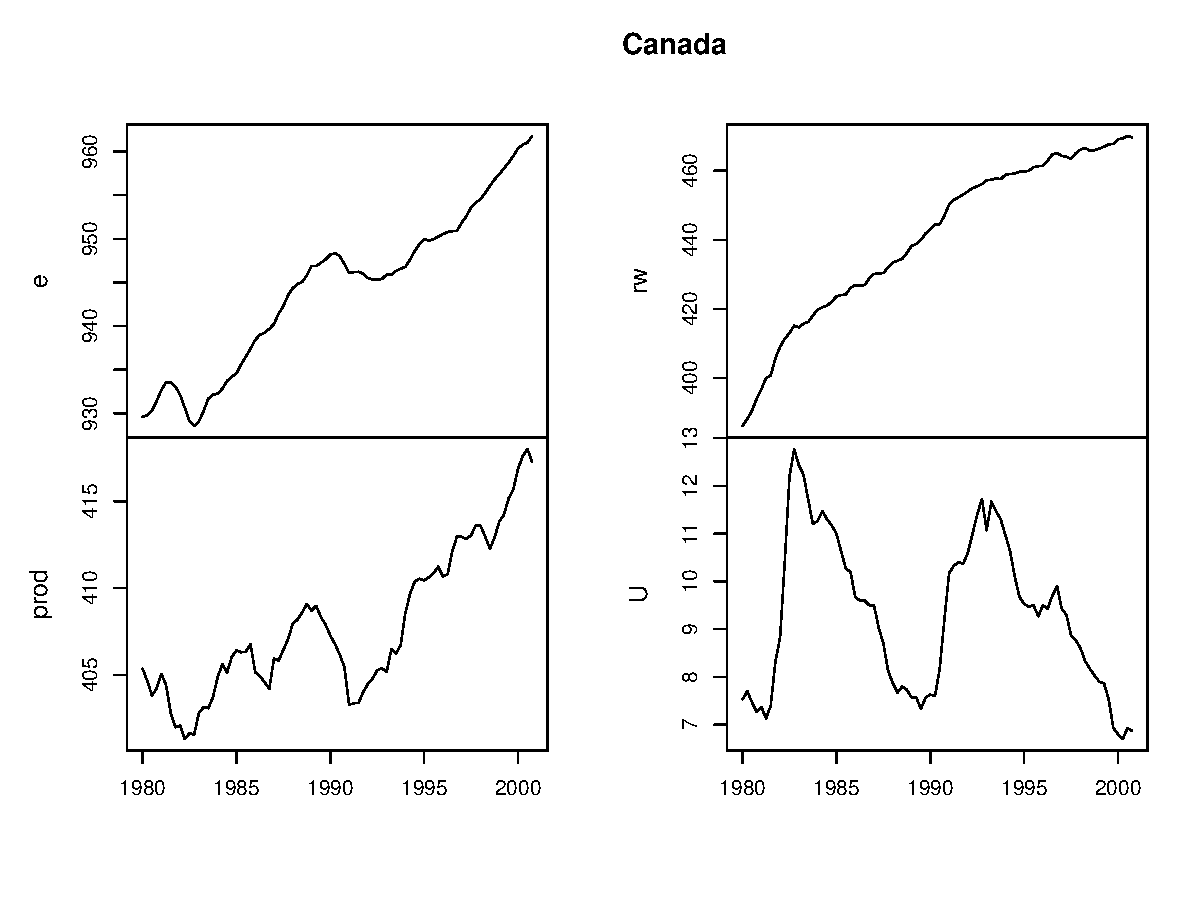
\includegraphics{Figures/fig-1}
\caption{Canadian labor market time series.}
\label{fig-1}
\end{figure}
%%
In a next step, the authors conducted unit root tests by applying
the Augmented Dickey-Fuller test regressions to the series (henceforth:
ADF~test). The ADF~test has been implemented in the package \pkg{urca} as
function \code{ur.df()}, for instance. The result of the ADF~tests are
summarized in Table~\ref{tab-2}.\footnote{In the following only
  \proglang{R}~code excerpts are shown. The \proglang{R}~code for
  producing the Tables and Figures below are provided in a separate
  file that accompanies this text.}   
%%
%% Example 2: Unit root tests
%% (Replication of Table 4.1)
%%
\begin{Schunk}
\begin{Sinput}
R> adf1 <- summary(ur.df(Canada[, "prod"], type = "trend", lags = 2))
R> adf1
\end{Sinput}
\begin{Soutput}
############################################### 
# Augmented Dickey-Fuller Test Unit Root Test # 
############################################### 

Test regression trend 


Call:
lm(formula = z.diff ~ z.lag.1 + 1 + tt + z.diff.lag)

Residuals:
    Min      1Q  Median      3Q     Max 
-2.1992 -0.3899  0.0429  0.4191  1.7166 

Coefficients:
            Estimate Std. Error t value Pr(>|t|)  
(Intercept) 30.41523   15.30940    1.99    0.051 .
z.lag.1     -0.07579    0.03813   -1.99    0.050 .
tt           0.01390    0.00642    2.16    0.034 *
z.diff.lag1  0.28487    0.11436    2.49    0.015 *
z.diff.lag2  0.08002    0.11609    0.69    0.493  
---
Signif. codes:  0 '***' 0.001 '**' 0.01 '*' 0.05 '.' 0.1 ' ' 1 

Residual standard error: 0.685 on 76 degrees of freedom
Multiple R-squared: 0.135,	Adjusted R-squared: 0.0899 
F-statistic: 2.98 on 4 and 76 DF,  p-value: 0.0244 


Value of test-statistic is: -1.9875 2.3 2.3817 

Critical values for test statistics: 
      1pct  5pct 10pct
tau3 -4.04 -3.45 -3.15
phi2  6.50  4.88  4.16
phi3  8.73  6.49  5.47
\end{Soutput}
\end{Schunk}
%%
\begin{Schunk}
\begin{Sinput}
R> adf2 <- summary(ur.df(diff(Canada[, "prod"]), type = "drift", 
+    lags = 1))
R> adf2
\end{Sinput}
\begin{Soutput}
############################################### 
# Augmented Dickey-Fuller Test Unit Root Test # 
############################################### 

Test regression drift 


Call:
lm(formula = z.diff ~ z.lag.1 + 1 + z.diff.lag)

Residuals:
    Min      1Q  Median      3Q     Max 
-2.0512 -0.3953  0.0782  0.4111  1.7513 

Coefficients:
            Estimate Std. Error t value Pr(>|t|)    
(Intercept)   0.1153     0.0803    1.44     0.15    
z.lag.1      -0.6889     0.1335   -5.16  1.8e-06 ***
z.diff.lag   -0.0427     0.1127   -0.38     0.71    
---
Signif. codes:  0 '***' 0.001 '**' 0.01 '*' 0.05 '.' 0.1 ' ' 1 

Residual standard error: 0.697 on 78 degrees of freedom
Multiple R-squared: 0.361,	Adjusted R-squared: 0.345 
F-statistic: 22.1 on 2 and 78 DF,  p-value: 2.53e-08 


Value of test-statistic is: -5.1604 13.318 

Critical values for test statistics: 
      1pct  5pct 10pct
tau2 -3.51 -2.89 -2.58
phi1  6.70  4.71  3.86
\end{Soutput}
\end{Schunk}
%%
\begin{table}
\begin{center}
\begin{tabular}{@{}lllllll@{}}
\toprule
\multicolumn{1}{l}{Variable}&
\multicolumn{1}{l}{Deterministic terms}&
\multicolumn{1}{l}{Lags}&
\multicolumn{1}{l}{Test value} &
\multicolumn{3}{c}{Critical values}
\\
\cmidrule(l){5-7}
& & & & 1\% & 5\% & 10\%\\
\midrule    
$\mathtt{prod}$ & constant, trend & 2 & $-$1.99 &
$-$4.04 & $-$3.45 & $-$3.15\\ 
$\varDelta \mathtt{prod}$ & constant & 1 & $-$5.16 &
$-$3.51 & $-$2.89 & $-$2.58\\ 
$\mathtt{e}$ & constant, trend & 2 & $-$1.91 &
$-$4.04 & $-$3.45 & $-$3.15\\ 
$\varDelta \mathtt{e}$ & constant & 1 & $-$4.51 &
$-$3.51 & $-$2.89 & $-$2.58\\ 
$\mathtt{U}$ & constant & 1 & $-$2.22 &
$-$3.51 & $-$2.89 & $-$2.58\\ 
$\varDelta \mathtt{U}$ & & 0 & $-$4.75 &
$-$2.60 &
$-$1.95 & $-$1.61\\  
$\mathtt{rw}$ & constant, trend & 4 & $-$2.06 &
$-$4.04 & $-$3.45 & $-$3.15\\ 
$\varDelta \mathtt{rw}$ & constant & 3 & $-$2.62 &
$-$3.51 & $-$2.89 & $-$2.58\\ 
$\varDelta \mathtt{rw}$ & constant & 0 & 
$-$5.60 &
$-$3.51 & $-$2.89 & $-$2.58\\ 
\bottomrule
\end{tabular}
\end{center}
\caption{ADF~tests for Canadian data.}
\label{tab-2}
\end{table}
%%
It can be concluded that all time series are integrated of order
one. Please note, that the reported critical values differ slightly
from the ones that are reported in \citet{BRE2004}. The authors
utilized the software \pkg{JMulTi} \citep{LUE2004} in which the
critical values of \cite{DAV1993} are used, whereas in the function
\code{ur.df()} the critical values are taken from \citet{DIC1981} and
\citet{HAM1994}.

In an ensuing step, the authors determined an optimal lag length for
an unrestricted VAR for a maximal lag length of eight. 
%%
%% Example 3: VAR selection
%% (last paragraph on page 189)
%%
\begin{Schunk}
\begin{Sinput}
R> VARselect(Canada, lag.max = 8, type = "both")
\end{Sinput}
\begin{Soutput}
$selection
AIC(n)  HQ(n)  SC(n) FPE(n) 
     3      2      1      3 

$criteria
                1          2          3          4          5          6
AIC(n) -6.2725791 -6.6366697 -6.7711769 -6.6346092 -6.3981322 -6.3077048
HQ(n)  -5.9784294 -6.1464203 -6.0848278 -5.7521604 -5.3195837 -5.0330565
SC(n)  -5.5365580 -5.4099679 -5.0537944 -4.4265460 -3.6993884 -3.1182803
FPE(n)  0.0018898  0.0013195  0.0011660  0.0013632  0.0017821  0.0020442
                7          8
AIC(n) -6.0707273 -6.0615969
HQ(n)  -4.5999792 -4.3947490
SC(n)  -2.3906220 -1.8908109
FPE(n)  0.0027686  0.0030601
\end{Soutput}
\end{Schunk}
According to the AIC and FPE the optimal lag number is $p=3$,
whereas the HQ criterion indicates $p=2$ and the SC criterion
indicates an optimal lag length of $p=1$. They estimated for all
three lag orders a VAR including a constant and a trend as
deterministic regressors and conducted diagnostic tests with respect
to the residuals. In the \proglang{R}~code example below, the relevant
commands are exhibited for the VAR($1$) model. First, the variables
have to be reordered in the same sequence as in \citet{BRE2004}. This
step is necessary, because otherwise the results of the multivariate
Jarque-Bera test, in which a Choleski decomposition is employed, would
differ slightly from the reported ones in \citet{BRE2004}. In the
\proglang{R}~code lines below the estimation of the VAR($1$) as well
as the summary output and the diagram of fit for equation ``\code{e}'' is shown. 
%%
%% Example 4: VAR estimation
%% (Replication of Table 4.2)
%%
\begin{Schunk}
\begin{Sinput}
R> Canada <- Canada[, c("prod", "e", "U", "rw")]
R> p1ct <- VAR(Canada, p = 1, type = "both")
R> p1ct
\end{Sinput}
\begin{Soutput}
VAR Estimation Results:
======================= 

Estimated coefficients for equation prod: 
========================================= 
Call:
prod = prod.l1 + e.l1 + U.l1 + rw.l1 + const + trend 

  prod.l1      e.l1      U.l1     rw.l1     const     trend 
 0.963137  0.012912  0.211089 -0.039094 16.243407  0.046131 


Estimated coefficients for equation e: 
====================================== 
Call:
e = prod.l1 + e.l1 + U.l1 + rw.l1 + const + trend 

    prod.l1        e.l1        U.l1       rw.l1       const       trend 
   0.194650    1.238923    0.623015   -0.067763 -278.761211   -0.040660 


Estimated coefficients for equation U: 
====================================== 
Call:
U = prod.l1 + e.l1 + U.l1 + rw.l1 + const + trend 

   prod.l1       e.l1       U.l1      rw.l1      const      trend 
 -0.123192  -0.248442   0.391580   0.065808 259.982010   0.034517 


Estimated coefficients for equation rw: 
======================================= 
Call:
rw = prod.l1 + e.l1 + U.l1 + rw.l1 + const + trend 

   prod.l1       e.l1       U.l1      rw.l1      const      trend 
 -0.223087  -0.051044  -0.368640   0.948909 163.024531   0.071422 
\end{Soutput}
\begin{Sinput}
R> summary(p1ct, equation = "e")
\end{Sinput}
\begin{Soutput}
VAR Estimation Results:
========================= 
Endogenous variables: prod, e, U, rw 
Deterministic variables: both 
Sample size: 83 
Log Likelihood: -207.525 
Roots of the characteristic polynomial:
0.95 0.95 0.904 0.751
Call:
VAR(y = Canada, p = 1, type = "both")


Estimation results for equation e: 
================================== 
e = prod.l1 + e.l1 + U.l1 + rw.l1 + const + trend 

         Estimate Std. Error t value Pr(>|t|)    
prod.l1    0.1947     0.0361    5.39  7.5e-07 ***
e.l1       1.2389     0.0863   14.35  < 2e-16 ***
U.l1       0.6230     0.1693    3.68  0.00043 ***
rw.l1     -0.0678     0.0283   -2.40  0.01899 *  
const   -278.7612    75.1830   -3.71  0.00039 ***
trend     -0.0407     0.0197   -2.06  0.04238 *  
---
Signif. codes:  0 '***' 0.001 '**' 0.01 '*' 0.05 '.' 0.1 ' ' 1 


Residual standard error: 0.47 on 77 degrees of freedom
Multiple R-Squared:    1,	Adjusted R-squared:    1 
F-statistic: 5.58e+07 on 6 and 77 DF,  p-value: <2e-16 



Covariance matrix of residuals:
         prod       e       U       rw
prod  0.46952  0.0677 -0.0413  0.00214
e     0.06767  0.2210 -0.1320 -0.08279
U    -0.04128 -0.1320  0.1216  0.06374
rw    0.00214 -0.0828  0.0637  0.59317

Correlation matrix of residuals:
         prod      e      U       rw
prod  1.00000  0.210 -0.173  0.00406
e     0.21008  1.000 -0.805 -0.22869
U    -0.17275 -0.805  1.000  0.23731
rw    0.00406 -0.229  0.237  1.00000
\end{Soutput}
\begin{Sinput}
R> plot(p1ct, names = "e")
\end{Sinput}
\end{Schunk}
%
\setkeys{Gin}{width=0.8\textwidth}
\begin{figure}[p]
\centering  
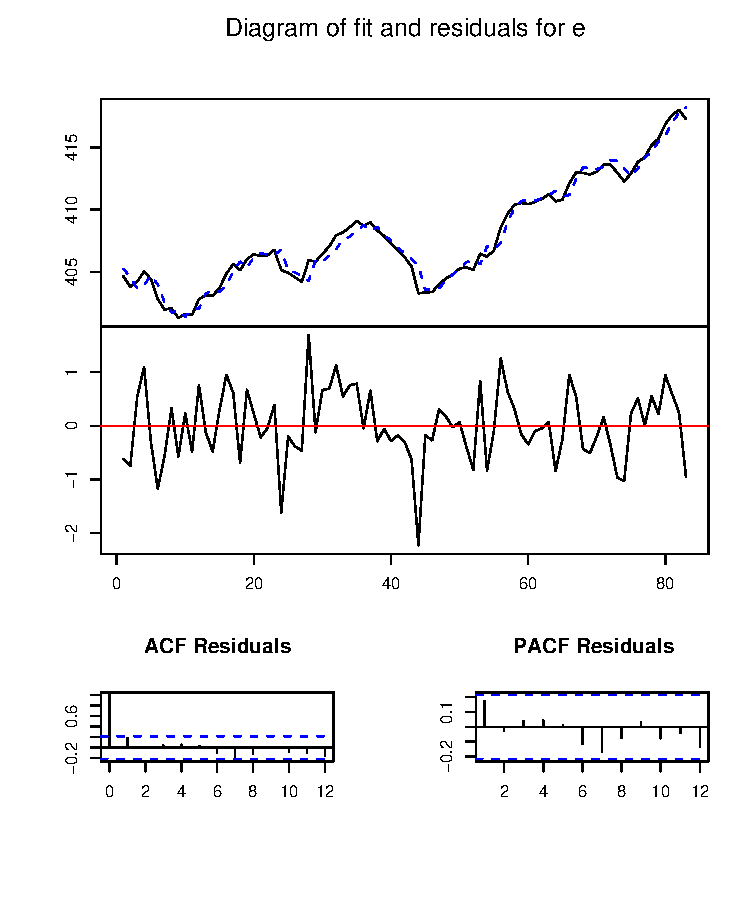
\includegraphics{Figures/fig-2}
\caption{Plot of VAR($1$) for equation ``\code{e}''.}
\label{fig-2}
\end{figure}
%%
%%
\begin{table}[p]
\begin{center}
\begin{tabular}{@{}lllllllll@{}}
\toprule
\multicolumn{1}{l}{Model}&
\multicolumn{1}{l}{$Q_{16}$}&
\multicolumn{1}{l}{$p$~value}&
\multicolumn{1}{l}{$Q_{16}^*$}&
\multicolumn{1}{l}{$p$~value}&
\multicolumn{1}{l}{$\textit{JB}_4$}&
\multicolumn{1}{l}{$p$~value}&
\multicolumn{1}{l}{$\textit{MARCH}_5$}&
\multicolumn{1}{l}{$p$~value}
\\
\midrule    
$p = 3$ & 174.0 &
0.96 & 
198.0 &
0.68 & 9.66 &
0.29 & 
512.0 &
0.35\\ 
$p = 2$ & 209.7 &
0.74 & 236.1 &
0.28 & 2.29 &
0.97 & 528.1 &
0.19\\ 
$p = 1$ & 233.5 &
0.61 & 256.9 &
0.22 & 9.92 &
0.27 & 570.1 &
0.02\\ 
\bottomrule
\end{tabular}
\end{center}
\caption{Diagnostic tests of VAR($p$) specifications for Canadian data.}
\label{tab-3}
\end{table}
%%
%%
The resulting graphic is displayed in Figure~\ref{fig-2}. Next, it is
shown how the diagnostic tests are conducted for the
VAR($1$) model. The results of all diagnostic tests, i.e., for the
VAR($1$), VAR($2$) and VAR($3$) model, are provided in
Table~\ref{tab-3} %%on page~\pageref{tab-3}
and the graphics of the
\code{varcheck} object \code{arch1} for the employment equation and the
OLS-CUSUM tests for the VAR($1$) model are shown in
Figures~\ref{fig-3} and \ref{fig-4}, respectively. 
%%
%%
\setkeys{Gin}{width=\textwidth}
\begin{figure}[p!]
\centering  
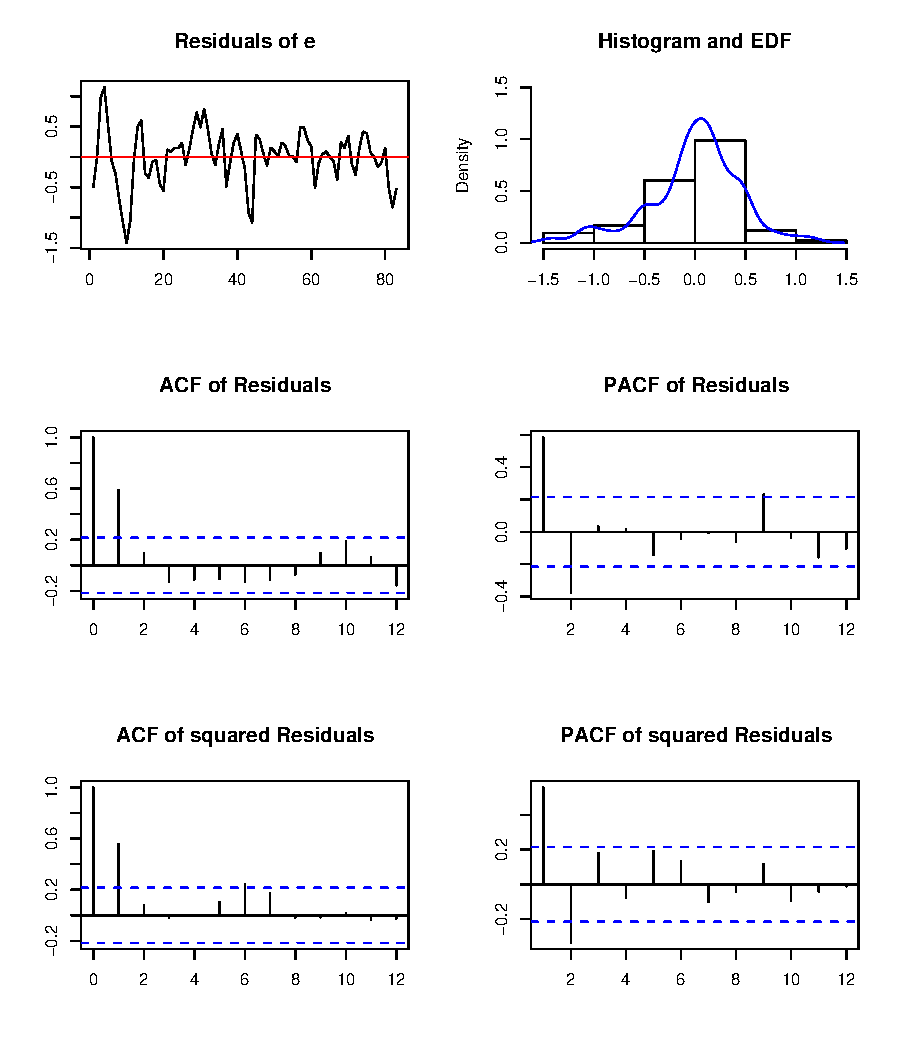
\includegraphics{Figures/fig-3}
\caption{Diagnostic plot of VAR($1$) for equation ``\code{e}''.}
\label{fig-3}
\end{figure}
%%
\setkeys{Gin}{width=\textwidth}
\begin{figure}[t!]
\centering  
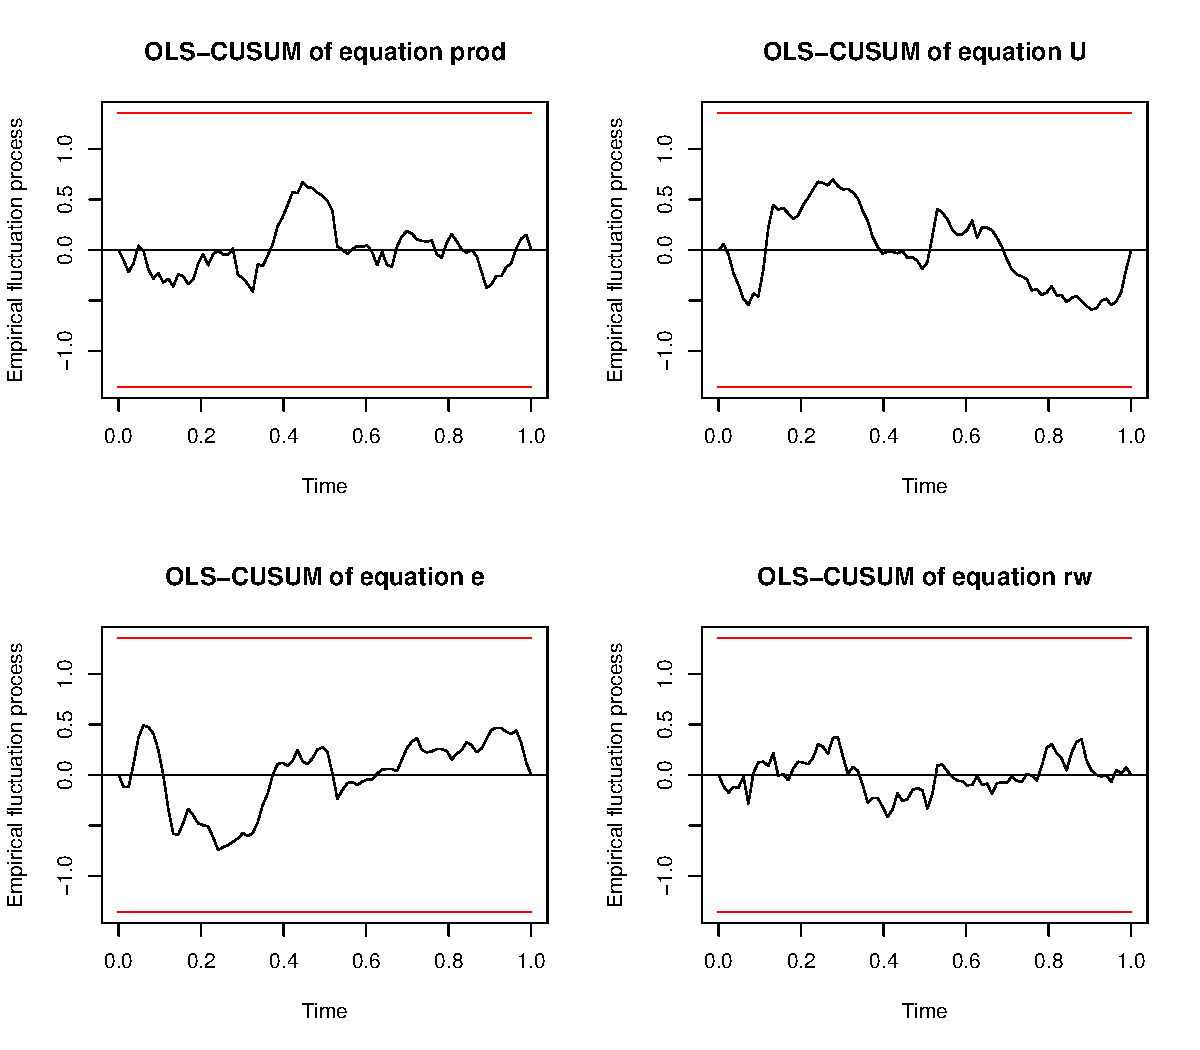
\includegraphics{Figures/fig-4}
\caption{OLS-CUSUM test of VAR($1$).}
\label{fig-4}
\end{figure}
%
\begin{Schunk}
\begin{Sinput}
R> ser11 <- serial.test(p1ct, lags.pt = 16, type = "PT.asymptotic")
R> ser11$serial
\end{Sinput}
\begin{Soutput}
	Portmanteau Test (asymptotic)

data:  Residuals of VAR object p1ct 
Chi-squared = 233.5, df = 240, p-value = 0.606
\end{Soutput}
\begin{Sinput}
R> norm1 <- normality.test(p1ct)
R> norm1$jb.mul
\end{Sinput}
\begin{Soutput}
$JB

	JB-Test (multivariate)

data:  Residuals of VAR object p1ct 
Chi-squared = 9.9189, df = 8, p-value = 0.2708


$Skewness

	Skewness only (multivariate)

data:  Residuals of VAR object p1ct 
Chi-squared = 6.356, df = 4, p-value = 0.1741


$Kurtosis

	Kurtosis only (multivariate)

data:  Residuals of VAR object p1ct 
Chi-squared = 3.5629, df = 4, p-value = 0.4684
\end{Soutput}
\begin{Sinput}
R> arch1 <- arch.test(p1ct, lags.multi = 5)
R> arch1$arch.mul
\end{Sinput}
\begin{Soutput}
	ARCH (multivariate)

data:  Residuals of VAR object p1ct 
Chi-squared = 570.14, df = 500, p-value = 0.01606
\end{Soutput}
\begin{Sinput}
R> plot(arch1, names = "e")
R> plot(stability(p1ct), nc = 2)
\end{Sinput}
\end{Schunk}
%%
Given the diagnostic test results the authors concluded that a
VAR($1$)-specification might be too restrictive. They argued further,
that although some of the stability tests do indicate deviations
from parameter constancy, the time-invariant specification of the
VAR($2$) and VAR($3$) model will be maintained as tentative candidates
for the following cointegration analysis. 
%%

The authors estimated a VECM whereby a deterministic trend has been
included in the cointegration relation. The estimation of these
models as well as the statistical inference with respect to the
cointegration rank can be swiftly accomplished with the function
\code{ca.jo()}. Although the following \proglang{R}~code examples are
using functions contained in the package \pkg{urca}, it is however
beneficial to reproduce these results for two reasons: the interplay
between the functions contained in package \pkg{urca} and \pkg{vars}
is exhibited and it provides an understanding of the then following
SVEC specification. 
%%
%% Example 5: VECM estimation I
%% (Replication of Table 4.3)
%%
\begin{Schunk}
\begin{Sinput}
R> summary(ca.jo(Canada, type = "trace", ecdet = "trend", K = 3, 
+    spec = "transitory"))
R> summary(ca.jo(Canada, type = "trace", ecdet = "trend", K = 2, 
+    spec = "transitory"))
\end{Sinput}
\end{Schunk}
%%
The outcome of the trace tests is provided in Table~\ref{tab-4}.
%%
%%
\begin{table}[t]
\begin{center}
\begin{tabular}{@{}lrrlll@{}}
\toprule
\multicolumn{1}{l}{}&
\multicolumn{2}{c}{Test Statistics}&
\multicolumn{3}{c}{Critical Values}
\\
\cmidrule(l){2-3}
\cmidrule(l){4-6}
\\
\multicolumn{1}{l}{$\mathcal{H}_0$}&
\multicolumn{1}{l}{$p = 3$}&
\multicolumn{1}{l}{$p = 2$}&
\multicolumn{1}{l}{90\%}&
\multicolumn{1}{l}{95\%}&
\multicolumn{1}{l}{99\%}
\\
\midrule    
$r = 0$ & 84.92 & 86.12 & 
59.14 & 62.99 & 70.05\\
$r = 1$ & 36.42 & 37.33 & 
39.06 & 42.44 & 48.45\\
$r = 2$ & 18.72 & 15.65 & 
22.76 & 25.32 & 30.45\\
$r = 3$ & 3.85 & 4.10 & 
10.49 & 12.25 & 16.26\\
\bottomrule
\end{tabular}
\end{center}
\caption{Johansen cointegration tests for Canadian system.}
\label{tab-4}
\end{table}
%%
These results do indicate one cointegration
relationship. The reported critical values differ slightly from the
ones that are reported in Table 4.3 of \citet{BRE2004}. The authors used
the values that are contained in \citet{JOH1995}, whereas the values from
\citet{OST1992} are used in the function \code{ca.jo()}. In the
\proglang{R}~code snippet below the VECM is re-estimated with this
restriction and a normalization of the long-run relationship with
respect to real wages. The results are shown in Table~\ref{tab-5}.   
%%
%% Example 6: VECM estimation II
%% (Replication of Table 4.4)
%%
\begin{Schunk}
\begin{Sinput}
R> vecm <- ca.jo(Canada[, c("rw", "prod", "e", "U")], type = "trace", 
+    ecdet = "trend", K = 3, spec = "transitory")
R> vecm.r1 <- cajorls(vecm, r = 1)
\end{Sinput}
\end{Schunk}
%%
%%
\begin{table}
\begin{center}
\begin{tabular}{@{}llllll@{}}
\toprule
\multicolumn{1}{l}{Vector}&
\multicolumn{1}{l}{$\mathtt{prod}$}&
\multicolumn{1}{l}{$\mathtt{e}$}&
\multicolumn{1}{l}{$\mathtt{U}$}&
\multicolumn{1}{l}{$\mathtt{rw}$}&
\multicolumn{1}{l}{$\mathrm{trend}$}
\\
\midrule    
$\hat{\bm{\beta}}^\top$ & 0.545 & $-$0.013 
& 1.727 & 1.000 & $-$0.709
\\
                    & (0.90) & ($-$0.02) 
& (1.19) &  & ($-$2.57)
\\

$\hat{\bm{\alpha}}^\top$ & $-$0.012 & $-$0.016 
& $-$0.009 & $-$0.085 &
\\
                     & ($-$0.92) & ($-$2.16) 
& ($-$1.49) & ($-$5.71) &
\\

\bottomrule
\end{tabular}
\end{center}
\caption{Cointegration vector and loading parameters (with $t$~statistics in parentheses).}
\label{tab-5}
\end{table}
%%
For a just identified SVEC model of type B one needs
$\frac{1}{2}K(K-1)=6$ linear independent restrictions. It is further
reasoned from the Beveridge-Nelson decomposition that there are $k^* =
r(K - r) = 3$ shocks with permanent effects and only one shock that
exerts a temporary effect, due to $r = 1$. Because the cointegration
relation is interpreted as a stationary wage-setting relation, the
temporary shock is associated with the wage shock variable. Hence, the
four entries in the last column of the long-run impact matrix $\Xi B$
are set to zero. Because this matrix is of reduced rank, only $k^* r =
3$ linear independent restrictions are imposed thereby. It is therefore
necessary to set $\frac{1}{2}k^*(k^*-1)=3$ additional elements to
zero. The authors assumed constant returns of scale and therefore
productivity is only driven by output shocks. This reasoning
implies zero coefficients in the first row of the long-run matrix for
the variables employment, unemployment and real wages, hence the
elements $\Xi B_{1, j}$ for $j = 2, 3, 4$ are set to zero. Because
$\Xi B_{1, 4}$ has already been set to zero, only two additional
restrictions have been added. The last restriction is imposed on the
element $B_{4, 2}$. Here, it is assumed that labor demand shocks do
not exert an immediate effect on real wages.

In the \proglang{R}~code example below the matrix objects \code{LR}
and \code{SR} are set up accordingly and the just-identified SVEC is
estimated with function \code{SVEC()}. In the call to the function
\code{SVEC()} the argument \code{boot = TRUE} has been employed such
that bootstrapped standard errors and hence $t$~statistics can be
computed for the structural long-run and contemporaneous coefficients.
%%
%% Example 7: SVEC
%% (Equations (4.33) and (4.34))
%%
\begin{Schunk}
\begin{Sinput}
R> vecm <- ca.jo(Canada[, c("prod", "e", "U", "rw")], type = "trace", 
+    ecdet = "trend", K = 3, spec = "transitory")
R> SR <- matrix(NA, nrow = 4, ncol = 4)
R> SR[4, 2] <- 0
R> LR <- matrix(NA, nrow = 4, ncol = 4)
R> LR[1, 2:4] <- 0
R> LR[2:4, 4] <- 0
R> svec <- SVEC(vecm, LR = LR, SR = SR, r = 1, lrtest = FALSE, boot = TRUE, 
+    runs = 100)
R> summary(svec)
\end{Sinput}
\begin{Soutput}
SVEC Estimation Results:
======================== 

Call:
SVEC(x = vecm, LR = LR, SR = SR, r = 1, lrtest = FALSE, boot = TRUE, 
    runs = 100)

Type: B-model 
Sample size: 81 
Log Likelihood: -161.838 
Number of iterations: 10 

Estimated contemporaneous impact matrix:
        prod       e        U     rw
prod  0.5840  0.0743 -0.15258 0.0690
e    -0.1203  0.2614 -0.15510 0.0898
U     0.0253 -0.2672  0.00549 0.0498
rw    0.1117  0.0000  0.48377 0.4879

Estimated standard errors for impact matrix:
       prod      e      U     rw
prod 0.0803 0.1047 0.2125 0.0660
e    0.0705 0.0596 0.1665 0.0402
U    0.0527 0.0433 0.0568 0.0309
rw   0.1462 0.0000 0.6142 0.0888

Estimated long run impact matrix:
       prod      e      U rw
prod  0.791  0.000  0.000  0
e     0.202  0.577 -0.492  0
U    -0.159 -0.341  0.141  0
rw   -0.153  0.596 -0.250  0

Estimated standard errors for long-run matrix:
      prod      e     U rw
prod 0.152 0.0000 0.000  0
e    0.230 0.1801 0.550  0
U    0.115 0.0884 0.149  0
rw   0.184 0.1549 0.264  0

Covariance matrix of reduced form residuals (*100):
       prod     e      U    rw
prod 37.464 -2.10 -0.251  2.51
e    -2.096 11.49 -6.927 -4.47
U    -0.251 -6.93  7.454  2.98
rw    2.509 -4.47  2.978 48.46
\end{Soutput}
\end{Schunk}
%%
%%
\begin{table}[t]
\begin{center}
\begin{tabular}{@{}lllll@{}}
\toprule
\multicolumn{1}{l}{Equation}&
\multicolumn{1}{l}{$\varepsilon_t^{\mathrm{gdp}}$}&
\multicolumn{1}{l}{$\varepsilon_t^{\mathrm{Labor}^d}$}&
\multicolumn{1}{l}{$\varepsilon_t^{\mathrm{Labor}^s}$}&
\multicolumn{1}{l}{$\varepsilon_t^{\mathrm{wage}}$}
\\
\midrule    
Output & 0.58 & 0.07 & $-$0.15 & 
0.07\\
& (7.28) & (0.71) & ($-$0.72) & 
(1.05)\\
Labor demand & $-$0.12 & 0.26 & $-$0.16 & 
0.09\\
& ($-$1.71) & (4.39) & ($-$0.93) & 
(2.23)\\
Unemployment & 0.03 & $-$0.27 & 0.01 & 
0.05\\
& (0.48) & ($-$6.16) & (0.10) & 
(1.61)\\
Real wages & 0.11 & 0.00 & 0.48 & 
0.49\\
& (0.76) &  & (0.79) & 
(5.50)\\
\bottomrule
\end{tabular}
\end{center}
\caption{Estimated coefficients of the contemporaneous impact matrix (with $t$~statistics in parentheses).}
\label{tab-6}
\end{table}
%%
%%

The results are summarized in the Tables~\ref{tab-6} and~\ref{tab-7}. The
values of the $t$~statistics differ slightly from the reported ones in
\citet{BRE2004} which can be attributed to sampling. In the
\proglang{R}~code example above only 100 runs have been executed,
whereas in \citet{BRE2004} 2000 repetitions have been used.
 
\begin{table}
\begin{center}
\begin{tabular}{@{}lllll@{}}
\toprule
\multicolumn{1}{l}{Equation}&
\multicolumn{1}{l}{$\varepsilon_t^{\mathrm{gdp}}$}&
\multicolumn{1}{l}{$\varepsilon_t^{\mathrm{Labor}^d}$}&
\multicolumn{1}{l}{$\varepsilon_t^{\mathrm{Labor}^s}$}&
\multicolumn{1}{l}{$\varepsilon_t^{\mathrm{wage}}$}
\\
\midrule    
Output & 0.79 & 0.00 & 0.00 & 
0.00\\
& (5.21) &  &  & \\
Labor demand & 0.20 & 0.58 & $-$0.49 & 
0.00\\
& (0.88) & (3.20) & ($-$0.89) & \\
Unemployment & $-$0.16 & $-$0.34 & 0.14 & 
0.00\\
& ($-$1.38) & ($-$3.86) & (0.95) & \\
Real wages & $-$0.15 & 0.60 & $-$0.25 & 
0.00\\
& ($-$0.83) & (3.85) & ($-$0.95) & \\
\bottomrule
\end{tabular}
\end{center}
\caption{Estimated coefficients of the long-run impact matrix (with $t$~statistics in parentheses).}
\label{tab-7}
\end{table}
%%

The authors investigated further if labor supply shocks do have no 
long-run impact on unemployment. This hypothesis is mirrored by
setting $\Xi B_{3, 3} = 0$. Because one more zero restriction has been
added to the long-run impact matrix, the SVEC model is now
over-identified. The validity of this over-identification restriction
can be tested with a LR test. In the \proglang{R}~code example below
first the additional restriction has been set and then the SVEC is
re-estimated by using the \code{upate} method. The result of the LR
test is contained in the returned list as named element \code{LRover}.
%%
%% Example 8: Overidentification test
%% (page 193, text below (4.34))
%%
\begin{Schunk}
\begin{Sinput}
R> LR[3, 3] <- 0
R> svec.oi <- update(svec, LR = LR, lrtest = TRUE, boot = FALSE)
R> svec.oi$LRover
\end{Sinput}
\begin{Soutput}
	LR overidentification

data:  vecm 
Chi^2 = 6.0745, df = 1, p-value = 0.01371
\end{Soutput}
\end{Schunk}
%%
The value of the test statistic is
6.07 and the $p$~value of this
$\chi^2(1)$-distributed variable is
0.014. Therefore, the null
hypothesis that shocks to the labor supply do not exert a long-run
effect on unemployment has to be rejected for a significance level of
5\%.

In order to investigate the dynamic effects on unemployment, the
authors applied an impulse response analysis. The impulse response
analysis shows the effects of the different shocks, i.e.,
output, labor demand, labor supply and wage, to unemployment. In the
\proglang{R}~code example below the \code{irf} method for objects with
class attribute \code{svecest} is employed and the argument \code{boot
  = TRUE} has been set such that confidence bands around the impulse
response trajectories can be calculated. 
%%
%% Example 9: IRF
%%
\begin{Schunk}
\begin{Sinput}
R> svec.irf <- irf(svec, response = "U", n.ahead = 48, boot = TRUE)
R> plot(svec.irf)
\end{Sinput}
\end{Schunk}
%%
The outcome of the IRA is exhibited in Figure~\ref{fig-5}.
 
%%
%% Figure 2: Replication of Figure 4.8
%%
\setkeys{Gin}{width=\textwidth}
\begin{figure}[t!]
\centering  
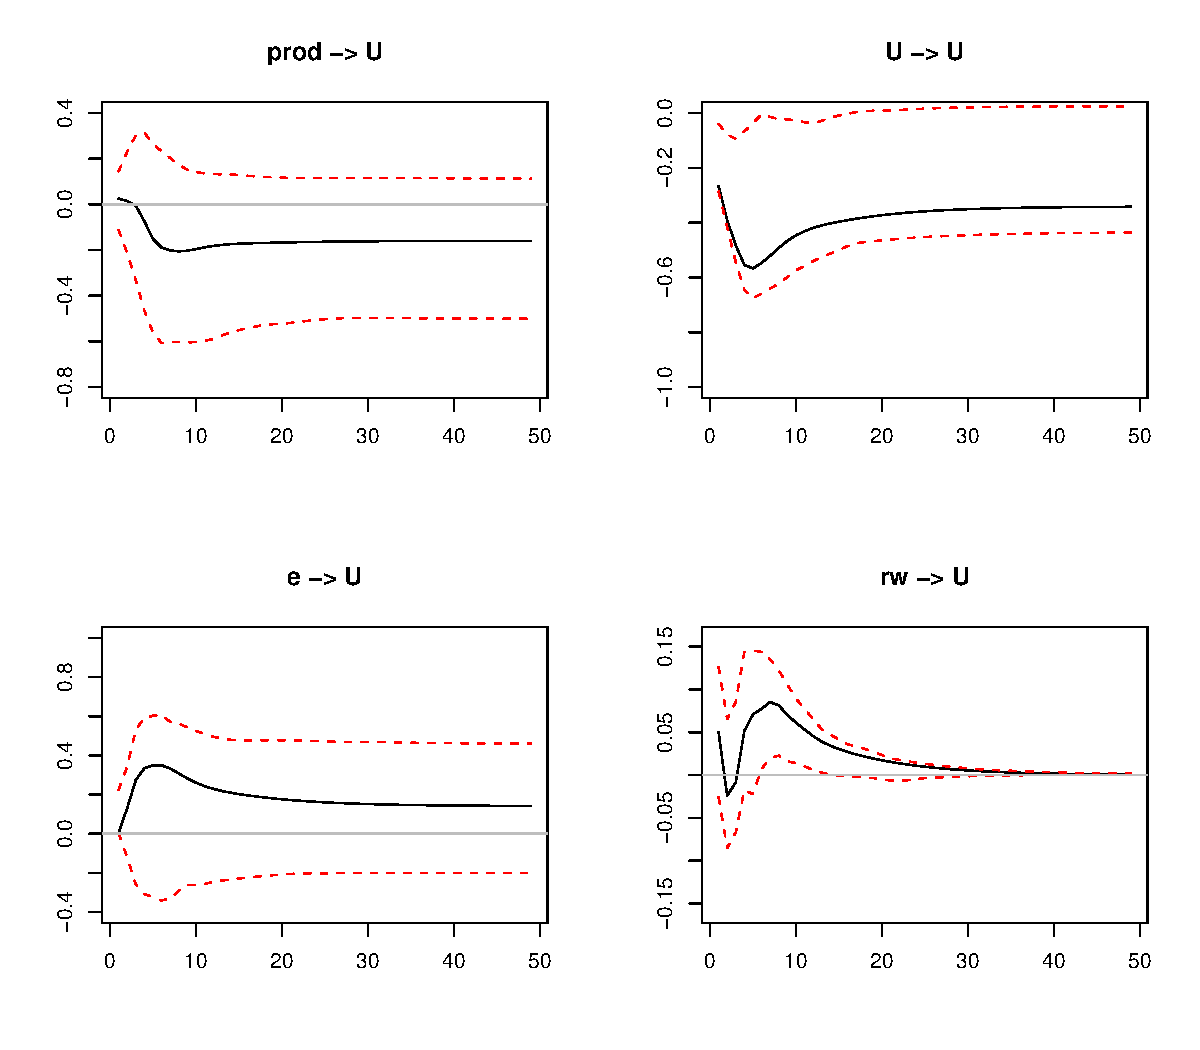
\includegraphics{Figures/fig-5}
\caption{Responses of unemployment to economic shocks with a $95$\%
  bootstrap confidence interval.}
\label{fig-5}
\end{figure}
%%

In a final step, a forecast error variance decomposition is conducted
with respect to unemployment. This is achieved by applying the
\code{fevd} method to the object with class attribute \code{svecest}.
%%
%% Example 9: FEVD
%% (Replication of Table 4.5)
%%
\begin{Schunk}
\begin{Sinput}
R> fevd.U <- fevd(svec, n.ahead = 48)$U
\end{Sinput}
\end{Schunk}
%%
The authors report only the values for selected quarters. These
results are displayed in Table~\ref{tab-8}.
%%
\begin{table}
\begin{center}
\begin{tabular}{@{}lllll@{}}
\toprule
\multicolumn{1}{l}{Period}&
\multicolumn{1}{l}{$\varepsilon_t^{\mathrm{gdp}}$}&
\multicolumn{1}{l}{$\varepsilon_t^{\mathrm{Labor}^d}$}&
\multicolumn{1}{l}{$\varepsilon_t^{\mathrm{Labor}^s}$}&
\multicolumn{1}{l}{$\varepsilon_t^{\mathrm{wage}}$}
\\
\midrule    
1 & 0.01 & 0.96 & 0.00 & 
0.03\\
4 & 0.01 & 0.78 & 0.21 & 
0.01\\
8 & 0.05 & 0.69 & 0.24 & 
0.01\\
12 & 0.08 & 0.68 & 0.23 & 
0.01\\
24 & 0.10 & 0.69 & 0.21 & 
0.01\\
48 & 0.12 & 0.70 & 0.18 & 
0.00\\
\bottomrule
\end{tabular}
\end{center}
\caption{Forecast error variance decomposition of Canadian unemployment.}
\label{tab-8}
\end{table}
%% 
%% Summary
%%
\newpage
\section{Summary}
\label{summary}
In this paper it has been described how the different functions and
methods contained in the package \pkg{vars} are designed and offer the
researcher a fairly easy to use environment for conducting VAR, SVAR and SVEC
analysis. This is primarily achieved through methods for impulse
response functions, forecast error variance decomposition, prediction
as well as tools for diagnostic testing, determination of a suitable
lag length for the model and stability / causality analysis.
 
The package \pkg{vars} complements the package \pkg{urca} in the sense that
most of the above described tools are available for VECM that can be
swiftly transformed to their level-VAR representation whence the
cointegrating rank has been determined.   

\section{Computational details} \label{sec:Appendix}

The package's code is purely written in \proglang{R}
\citep{R2006} and \proglang{S}3-classes with methods have been
utilized. It is shipped with a \code{NAMESPACE} and a \code{ChangeLog} file. It has
dependencies to \pkg{MASS} \citep{MASS}, \pkg{strucchange}
\citep{strucchange} and \pkg{urca}
\citep{urca}. \proglang{R} itself as well as these packages can
be obtained from CRAN at \url{http://CRAN.R-project.org/}. Furthermore, daily
builds of package \pkg{vars} are provided on \proglang{R}-Forge (see
\url{http://R-Forge.R-project.org/projects/vars/}). It has been published under
GPL version~2 or newer. The results used in this paper were obtained using \proglang{R} 
2.7.0 with
packages \pkg{vars} 1.3-8,
\pkg{strucchange} 1.3-3,
\pkg{urca} 1.1-6 and \pkg{MASS}
7.2-42.  

\section*{Acknowledgments}
I would like to thank the anonymous reviewers and Achim Zeileis for
valuable feedback on this article as well as the suggested
improvements for package \pkg{vars}.

\clearpage

\bibliography{vars}

\end{document}

